Inspired by a simpler structure in BigTable\citep{BigTable}, 
LevelDB \citep{LevelDB} is an open-source key-value storage library
that features an Log-Structured Merge (LSM) Tree \citep{ONeil1996} for on-disk storage.
In a simple understanding of an LSM tree, an in memory buffer cache delays 
writing new and changed entries until it has a significant amount of change to record on disk.
Using LevelDB as a local storage representation for metadata, 
can transform metadata updates to large, non-overwrite, sorted and indexed logs on disks,
which greatly reduces random disk seeks.
The detailed design of LevelDB and how to use LevelDB to store metadata is explained as the follows.

\subsubsection*{LevelDB and LSM Tree. }

%\begin{figure}[!ht]
\begin{figure}[t]
\centering
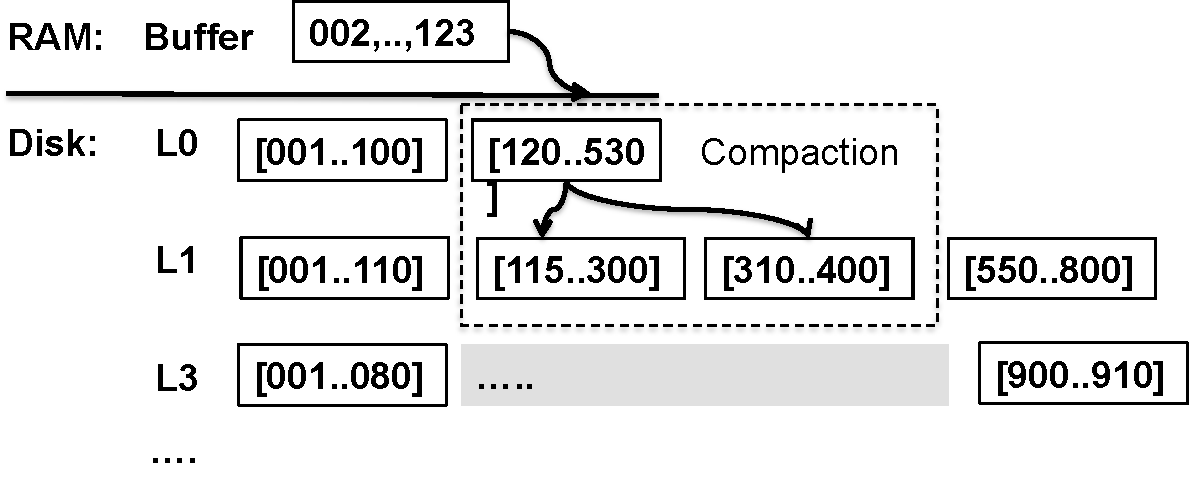
\includegraphics[scale=0.4]{figs/leveldb}
\caption{LevelDB represents data on disk in multiple SSTables that store sorted key-value pairs.}
\vspace{10pt}
\hrule 
\label{fig:leveldb}
\end{figure}


In LevelDB, by default, a set of changes are spilled to disk when the total size of modified entries exceeds 4 MB.  When a spill is triggered, called a minor compaction, the changed entries are sorted, indexed and written to disk in a format called an SSTable\citep{BigTable}.  These entries may then be discarded by the in memory buffer and can be reloaded by searching each SSTable on disk, possibly stopping when the first match occurs if the SSTables are searched most recent to oldest.  The number of SSTables that need to be searched can be reduced by maintaining a Bloom filter\citep{bloomfilter} on each, but with time the cost of finding a record not in memory increases.  Major compaction, or simply ``compaction", is the process of combining multiple SSTables into a smaller number of SSTables by merge sort. 

As illustrated in Figure \ref{fig:leveldb}, LevelDB extends this simple approach to further reduce read costs by dividing SSTables into sets, or levels.
The 0-th level of SSTables may contain entries with any key value, based on what was in memory at the time of its spill.
The higher levels of LevelDB's SSTables are the results of compacting SSTables from their own or lower levels.
In these higher levels, LevelDB maintains the following invariant: the key range spanning each SSTable is disjoint from the key range of all other SSTables at that level.
So querying for an entry in the higher levels only need read at most one SSTable in each level.
LevelDB also sizes each of the higher levels differentially:  all SSTables have the same maximum size and the sum of the sizes of all SSTables at level $L$ will not exceed $10^L$ MB.
This ensures that the number of level grows logarithmically with increasing numbers of entries.

\subsubsection*{Table Schema. } 

The local metadata store aggregates directory entries, 
inode attributes into one LevelDB table with a row for each file / directory.
To link together the hierarchical structure of the user's namespace,
the rows of the table are ordered by a 224-bit key consisting of 
the 64-bit inode number of a file's parent directory 
and a 160-bit SHA-1 hash value of its filename string (final component of its pathname).
The value of a row contains the file's full name and inode attributes,
such as inode number, ownership, access mode, file size, timestamps (\textit{struct stat} in Linux),
and a symbolic link that contains the actual path of the file object in the object store.
Figure \ref{fig:schema} shows an example of storing a sample file system's metadata into one LevelDB table.

%\begin{figure}[!ht]
\begin{figure}[t]
\centering
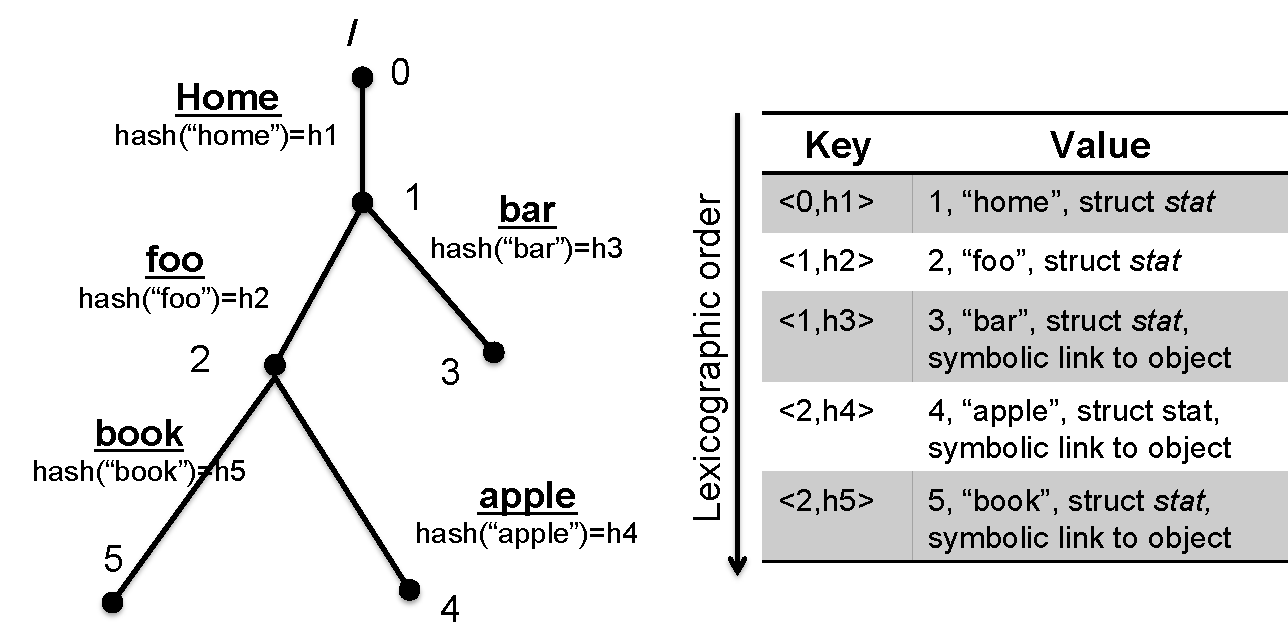
\includegraphics[scale=0.35]{figs/schema}
\caption{An example illustrates table schema for storing metadata into LevelDB.}
\vspace{10pt}
\hrule 
\label{fig:schema}
\end{figure}

All the entries in the same directory have rows that 
share the same first 64 bits in their the table's key.
For $readdir$ operations, once the inode number
of the target directory has been retrieved, 
a scan sequentially lists all entries having 
the directory's inode number as the first 64 bits of their table's key. 
To resolve a single pathname, the metadata server starts searching from the root inode, 
which has a well-known global inode number $(0)$.
Traversing the user's directory tree
involves constructing a search key by concatenating the inode 
number of current directory with the hash of
next component name in the pathname.
